\documentclass[12pt,a4paper]{article} 
%%%%%%%%%%%%%%%%%%%%%%%%%%%%%%%%%%%%%%%%%%%%%%%%%%%%%%%%%%%
% Preamble, everything that is inserted here is only for the computer to know what and how to compile the output. If you are not sure what you are doing, refrain from changing stuff
%%%%%%%%%%%%%%%%%%%%%%%%%%%%%%%%%%%%%%%%%%%%%%%%%%%%%%%%%%%
\usepackage[utf8]{inputenc} % this packages for example (inputenc) with the option utf8, lets us use special utf-8 characters (f.e., ä, ü, ö, ß, etc)
\usepackage{amsmath} % for beautiful math symbols 
\usepackage{amsfonts} % for nicer fonts
\usepackage{amssymb} % for nicer symbols
\usepackage[all]{nowidow} % to avoid widows and clubs, see also: http://www.tex.ac.uk/FAQ-widows.html
\usepackage[style=authoryear, backend=biber, maxnames=3]{biblatex} % for the citation, change style if you want
% examples can be found here:
% https://www.sharelatex.com/learn/Biblatex_citation_styles
% and
% https://www.sharelatex.com/learn/Biblatex_bibliography_styles
\usepackage[all]{nowidow} % google widows and orphans latex... 
\usepackage{hyperref} % add [hidelinks] if you don't want to see each link highlighted...
\usepackage[pdftex]{graphicx} % if you want to include pdfs 
%\usepackage[ngerman]{babel} % For German proofing, a German "Abbildungsverzeichnis" instead of an English List of Figures etc...
\usepackage[onehalfspacing]{setspace} % to get more spacing 
\addbibresource{bib_file.bib} % This points LaTeX to the right .bib file for the bibliography
\setlength\parindent{0pt} % no paragraph indent
%\DefineBibliographyStrings{ngerman}{andothers = {{et\,al\adddot}},} % comment this out if you are writing in English, furthermore, comment the babel package out
% you might have to recompile the file(s) afterwards (the magic trick for every error)



%%%%%%%%%%%%%%%%%%%%%%%%%%%%%%%%%%%%%%%%%%%%%%%%%%%%%%%%%%%
% Document, everything after \begin{document} will be included as text or other content in the document
%%%%%%%%%%%%%%%%%%%%%%%%%%%%%%%%%%%%%%%%%%%%%%%%%%%%%%%%%%%
% the only exception is a line starting with a %, which is a comment (disregarded by the compiler)

% change the following to match your needs
\newcommand{\Title}{A Minimal Working Example for a Master Thesis} 
% i.e., \newcommand{\Title}{A Theoretical Evaluation of the Effect of Potatoes on the Dynamic Allocation of Goods} (if thats your title)

\newcommand{\Degree}{Master of Science}
\newcommand{\Programme}{Corporate Management \& Economics}
\newcommand{\Name}{Max Mustermann}
\newcommand{\MatrikelNummer}{12345678}
\newcommand{\Date}{01-12-2015}
\newcommand{\Semester}{Fall Term 2016}
\newcommand{\Supervisor}{Prof. Dr. Marcel Tyrell}
\newcommand{\Pruefer}{Zweitgutachter}
\newcommand{\Chair}{Institute for Entrepreneurship \& Finance}

\begin{document}
%%%%%%%%%%%%%%%%%%%%%%%%%%%%%%%%%%%%%%%%%%%%%%%%%%%%%%%%%%%
% Title Page with logo and name
%%%%%%%%%%%%%%%%%%%%%%%%%%%%%%%%%%%%%%%%%%%%%%%%%%%%%%%%%%%

\pagenumbering{gobble}
\begin{centering}
\Large \textbf{Zeppelin Universität}\\
\Large \Chair \\
\vfill
\LARGE \textbf{\Title} \\
\vfill
\LARGE \Degree\\ %Bachelorarbeit
\Large in \\
\LARGE \Programme\\
\vfill
\begin{small}
\begin{doublespace}
	\begin{tabbing}
	Immatrikulationsnummerrrrr\=\kill
	Bearbeitet von:\>\Name\\
	Immatrikulationsnummer:\>\MatrikelNummer\\
	Studiengang:\>\Programme\\
	Semester:\>\Semester\\
	Betreuer:\>\Supervisor\\
	Prüfer:\>\Pruefer\\
	Abgabedatum:\>\Date
	\end{tabbing}
\end{doublespace}
\end{small}

\end{centering}\vspace{1cm}
\newpage

\pagenumbering{roman}
%%%%%%%%%%%%%%%%%%%%%%%%%%%%%%%%%%%%%%%%%%%%%%%%%%%%%%%%%%%
% Table of Contents, etc
%%%%%%%%%%%%%%%%%%%%%%%%%%%%%%%%%%%%%%%%%%%%%%%%%%%%%%%%%%%
% TOC (Tabel of Contents) are created automatically, by taking every \section, \subsection etc,
\tableofcontents
\listoffigures
\listoftables

\newpage

%%%%%%%%%%%%%%%%%%%%%%%%%%%%%%%%%%%%%%%%%%%%%%%%%%%%%%%%%%%
% Abstract
%%%%%%%%%%%%%%%%%%%%%%%%%%%%%%%%%%%%%%%%%%%%%%%%%%%%%%%%%%%
\pagenumbering{arabic}

\section{Abstract}
Here comes the English abstract!

\vfill % that the upper paragraph stays at the top, the lower one at the bottom

\section*{Kurzzusammenfassung} % the "*" takes out the numbering of the section (it also doesnt show up in the table of contents

Hier kommt das deutsche Abstrakt hin!

\newpage

%%%%%%%%%%%%%%%%%%%%%%%%%%%%%%%%%%%%%%%%%%%%%%%%%%%%%%%%%%%
% Introduction, by the way, these comments are only here for the writer to comment on something, if you want to use this for your project, delete everything after this until the %%%%%%%Bibliography%%%%%%%%%%
%%%%%%%%%%%%%%%%%%%%%%%%%%%%%%%%%%%%%%%%%%%%%%%%%%%%%%%%%%%

\section{Introduction}
BURN AFTER READING. 

I.e., everything that follows can be deleted up until the command 'printbibliography'.

\subsection{Minimal Working Example Citation}
A usual citation looks like this \parencite{R2016}. Whereas, a direct citation looks like this: \textcite{Hlavac2015} approves (hopefully). The bibliography is compiled automatically using the bib-file (in this case called 'bib\_file.bib'). To add additional sources add the bibtex code for the sources into the bib-file. More information about citation can be found in this \href{https://en.wikibooks.org/wiki/LaTeX/Bibliography_Management#biblatex}{Wikibook (click me)}, just make sure that you use biblatex and not bibtex (there is a difference!).\\

The code for the bib\_file can be also obtained from scholar.google.com, i.e., search for 'Modigliani Miller 1958' (\href{https://scholar.google.de/scholar?hl=en&q=modigliani+miller+1958&btnG=&as_sdt=1%2C5&as_sdtp=}{result of the search (click me)}) and then click on 'cite' and then 'BibTeX' (in this case biblatex and bibtex behave the same), which results in this 
\begin{verbatim}
@article{modigliani1958cost,
  title={The cost of capital, corporation finance and the theory of investment},
  author={Modigliani, Franco and Miller, Merton H},
  journal={The American economic review},
  volume={48},
  number={3},
  pages={261--297},
  year={1958},
  publisher={JSTOR}
}
\end{verbatim}

that can be directly copied to the bib\_file (though you might want to change the key from 'modigliani1958cost' to 'Modigliani1958' or something like this, just make sure that you refer to the right key!).\\

To compile the document with the citations you need to compile it using 'PdfLaTeX - BibTex(biber) - (2x) PdfLaTeX' (or you can change that in the 'quick-build' option in the Options). Make sure that you have biber installed and working. If it's not working check these options out (using Texmaker):
Go to 'Options' $\rightarrow$ 'Configure Texmaker' $\rightarrow$ 'Commands' $\rightarrow$ edit the field 'Bib(la)tex' to:
\begin{itemize}
\item MAC: biber \%.bcf \\
If not working check this \href{http://tex.stackexchange.com/questions/153359/setting-up-texmaker-on-mac-to-work-with-biber}{SO-question (click me)}
\item Win: "C:/Program Files (x86)/MiKTeX 2.9/miktex/bin/biber.exe" \%\\
Or wherever your miktex is installed. If this is not working check this \href{http://tex.stackexchange.com/questions/63039/install-biber-in-miktex-on-a-64-bit-version-of-windows}{SO-question (click me)})
\end{itemize}

For the sake of completeness I also cite a book by \textcite{Wilkinson2006}, an article by two \textcite{Modigliani1958}, as well as another article by three \textcite{Johnson2000}. Last tip, if it shows up like this \textcite{UnknownKey2000}, that means the key for the citation is not found!

\subsection{Minimal Working Example Pictures}
Pictures look like this (caption above, description below, centered image, relative size to text may vary depending on your needs). If you have questions refer to \href{https://en.wikibooks.org/wiki/LaTeX/Floats,_Figures_and_Captions}{this Wikibook (click me)}

\begin{figure}[h]
\centering
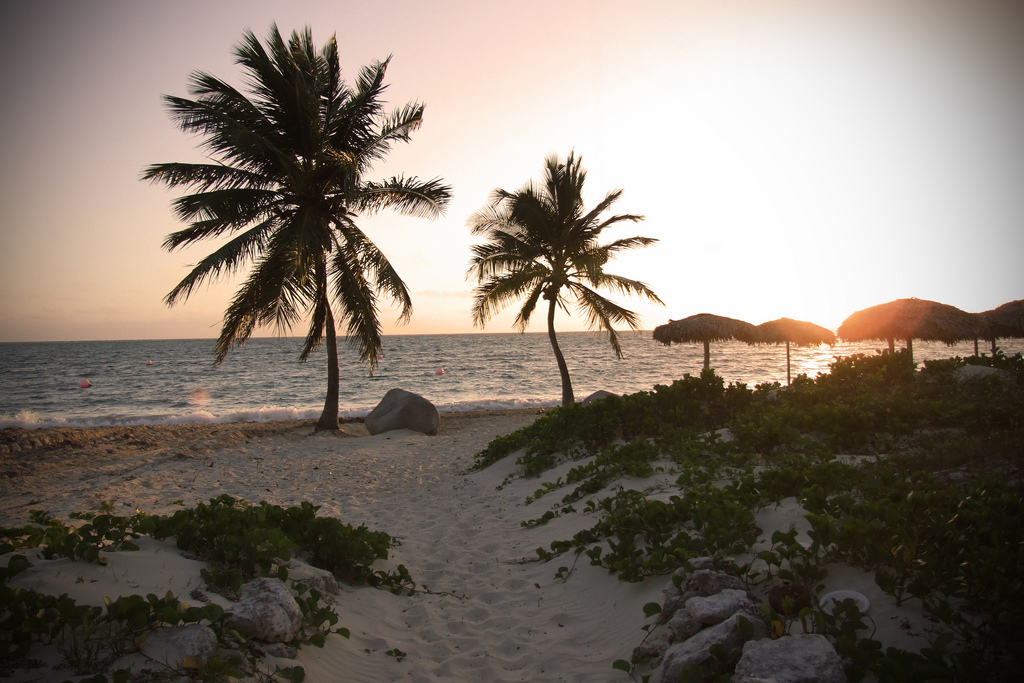
\includegraphics[width=0.5\textwidth]{pictures/beach.jpg} \\
\caption{Image captions go below the image (usually)}
\small Some more information if necessary.
\end{figure}


\subsection{Minimal Working Example Math}
\label{subsec:math}
A math equation is centered and numbered which looks like this:

\begin{equation}
a = \sqrt{b^2 + c^2}.
\end{equation}

If possible align equations (if you use multiple equations per equation-float):

\begin{equation}
\begin{split}
a &= \sqrt{b^2 + c^2}\\
b &= \sqrt{a^2 - b^2} + 100 - 100 
\end{split}
\end{equation}

There is the possibility of having inline-math which looks like this $\lambda = 1 - x$, but refrain from abusing it to look like this: $\mu = \displaystyle \sum_{i = 1}^{n} \frac{x}{n}$ (inline).

For more information regarding math in \LaTeX, please refer to \href{https://en.wikibooks.org/wiki/LaTeX/Mathematics}{this Wikibook (click me)}

\subsection{Minimal Working Example Tables}
Tables should be saved in a separate file to keep the source-file (i.e., the document that you compile) tidy.\\

A table looks like \autoref{tab:Table1} (keep in mind that \LaTeX \ decides for you where to put the table, you can specify parameters such as '[h!]' ('h' for here, 'b' for bottom of the page, 't' for top, and 'p' for appendix. An '!' adds weight to a single parameter; you can also chain commands such as '[htbp]'. Because of pushing-around, make sure that you use references as described in \autoref{subsec:references}). \\

\begin{table}[h!]
\centering
\caption{Table captions go above the table (usually)}
\label{tab:Table1}
\begin{tabular}{l c }
	\hline
	& Model 1 \\
	\hline
	The Intercept & $4045.33^{***}$ \\
	& $(286.21)$      \\
	Depth         & $-102.17^{***}$ \\
	& $(4.64)$        \\
	Carat         & $7765.14^{***}$ \\
	& $(14.01)$       \\
	\hline
	R$^2$         & 0.85            \\
	Adj. R$^2$    & 0.85            \\
	Num. obs.     & 53940           \\
	RMSE          & 1541.65         \\
	\hline
	\multicolumn{2}{l}{\scriptsize{$^{***}p<0.001$, $^{**}p<0.01$, $^*p<0.05$}}
\end{tabular}
\\
\bigskip
\small Additional Information can be supplied here in the form of free text! If you want to have the same width as the table, include a row in the table itself!
\end{table}

Regression results should be exported automatically, i.e., using the r-packages stargazer, texreg, xtable or some other alternative. The code to produce the table shown, is in the appendix in \autoref{sec:appendix}. \\

For more information regarding tables in \LaTeX, please refer to \href{https://en.wikibooks.org/wiki/LaTeX/Tables}{this Wikibook (click me)}. If you have a long table, use the longtable latex-package!
\newpage

\subsection{Referencing Examples}
\label{subsec:references}
If possible, use the power of \LaTeX \ to automatically reference. I.e., to refer to \autoref{subsec:math} (the Maths subsection) or to \autoref{tab:Table1} (in Texmaker you see red boxes around the links, these disappear in the PDF-print, if you want to disable them at all, include the '[hidelinks]' parameter to the usepackage-hyperref-command in the preamble in line 16).

%\section{Theoretical Concepts}

%\section{Data}
%Here goes the data.

%\section{Methods}
%Here go the methods

%\section{Results}
%Here go the results.

%\section{etc}
% add what you like/need

\newpage

%%%%%%%%%%%%%%%%%%%%%%%%%%%%%%%%%%%%%%%%%%%%%%%%%%%%%%%%%%%
% Bibliography
%%%%%%%%%%%%%%%%%%%%%%%%%%%%%%%%%%%%%%%%%%%%%%%%%%%%%%%%%%%
\printbibliography

\newpage

%%%%%%%%%%%%%%%%%%%%%%%%%%%%%%%%%%%%%%%%%%%%%%%%%%%%%%%%%%%
% Appendix
%%%%%%%%%%%%%%%%%%%%%%%%%%%%%%%%%%%%%%%%%%%%%%%%%%%%%%%%%%%
\section{Appendix: R-Code to create the tables}
\label{sec:appendix}
\begin{verbatim}
library(stargazer)
library(ggplot2) # for the data only

# create a regression
reg_result <- lm(data = diamonds, price ~ carat + depth + x + y + z)

# save the result to a tex file using stargazer
stargazer(reg_result, float = F, out = "reg_result.tex")

# make sure to either copy the file to tables/ or insert the path directly
# a direct path could look like this
# out = "C:/Documents/myWork/paper/tables/reg_result.tex"
\end{verbatim}

\newpage
\section*{Eidesstattliche Erklärung}

%Hiermit versichere ich, dass die vorliegende Arbeit selbstständig von mir in Übereinstimmung mit den Universitätsrichtlinien und mit keinen anderen als den angegebenen Quellen und Hilfsmitteln verfasst wurde. Alle Ausführungen, die aus anderen Schriften, Reden, Filmen oder sonstigen Quellen wörtlich oder sinngemäß entnommen wurden, sind als diese kenntlich gemacht. \\
%
%Weiterhin versichere ich, dass die vorliegende Arbeit nicht in gleicher oder ähnlicher Fassung Bestandteil einer anderen Studien- oder Prüfungsleistung war oder ist.\\

Hiermit erkläre ich, dass die vorliegende Arbeit in Übereinstimmung mit den Universitätsrichtlinien erstellt wurde und nicht in gleicher oder ähnlicher Fassung Bestandteil einer anderen Studien- oder Prüfungsleistung ist. Die Arbeit wurde mit keinen anderen als den angegebenen Quellen und Hilfsmitteln verfasst. Sollten Teile der Arbeit in Zusammenarbeit oder mit fremder Hilfe erstellt worden sein, so ist dies ausreichend gekennzeichnet. Die in der Arbeit vertretenden Meinungen sind die des Autors.\\

\section*{Author's Declaration}

I hereby declare that the work in this dissertation was carried out in accordance with the requirements of the university's regulations and that it has not been submitted for any other academic award. Except where indicated by specific references in the text, the work is the candidate's own work. Work done in collaboration with, or with the assistance of others, is indicated as such. Any views expressed in the dissertation are those of the author.

\vspace{3 cm}


\begin{tabular}{ll}
\makebox[0.3\textwidth]{\hrulefill} & \makebox[0.6\textwidth]{\hrulefill}\\
Ort, Datum & Unterschrift der Verfasserin/des Verfassers\\
Place, Date & Signature of the author\\
\end{tabular}

\end{document}




